% !TEX root = ../../main.tex

\subsection{Nitrogen sorption at 77K}

Isotherms have been recorded on samples activated at 
\SI{200}{\degreeCelsius}.
It is important to note that, as seen from the TGA curves,
not all capping agents leave the structure when thermal treating 
at this temperature. The modulator which is still present 
within the pore surface will likely influence the adsorption
behaviour.

Several example isotherms can be found in 
\autoref{def:fgr:n2phys-dataset}, with the complete dataset 
present in \autoref{appx:def}, \autoref{appx:def:tga}.

Several isotherm features can be analysed to assess the 
type of modifications introduced in the structure and their
preponderence:

\begin{itemize}
    \item the slope of the isotherm at low \(p/p_0\) is representative
    of the first interactions with the pore surface, which can be
    quantified using the initial Henry constant;
    \item missing liker defects will lead to an increase of the 
    apparent surface area;
    \item the pore size distribution and total pore volume give 
    indications on the presence of missing cluster defects and/or
    of the formation of mesoporous voids within the structure;
    \item a steep slope at high \(p/p_0\) is indicative of intercrystal
    condensation and suggests particle aggregation due to lower average 
    crystal size.
\end{itemize}

\begin{figure}[htbp]
    \centering

    \begin{subfigure}{0.45\linewidth}
        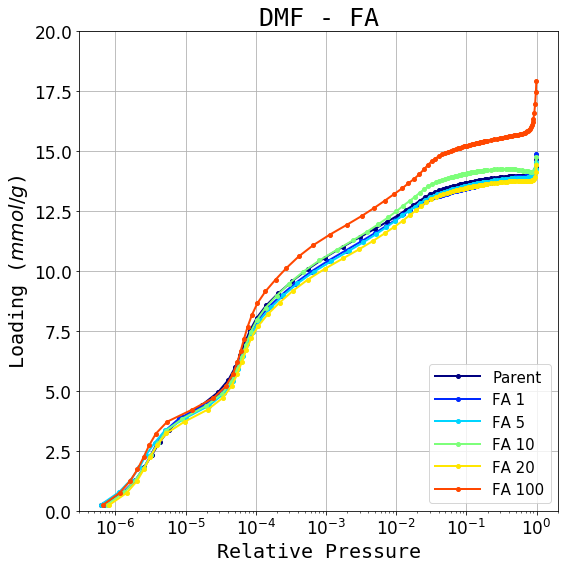
\includegraphics[width=\textwidth]{n2phys/dmf-fa}%
		\caption{}%
        \label{def:fgr:n2phys-dmf-fa}
    \end{subfigure}
    \begin{subfigure}{0.45\linewidth}
        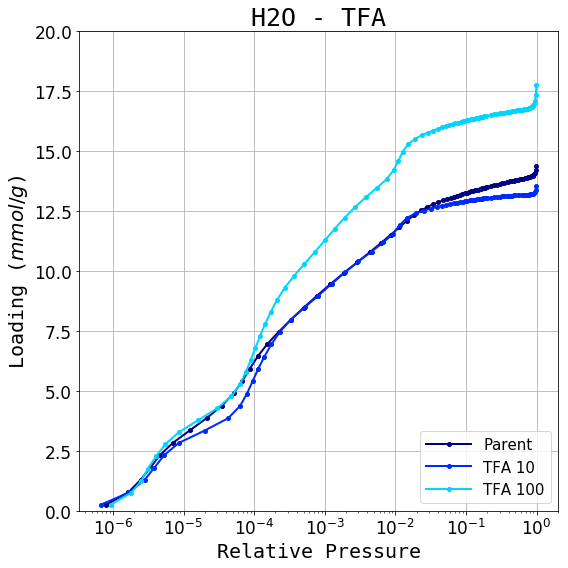
\includegraphics[width=\textwidth]{n2phys/h2o-tfa}%
		\caption{}%
        \label{def:fgr:n2phys-h2o-tfa}
    \end{subfigure}

    
    \begin{subfigure}{0.45\linewidth}
        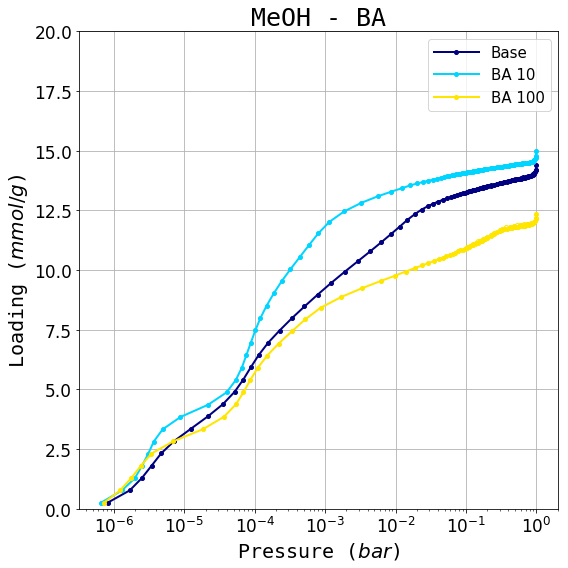
\includegraphics[width=\textwidth]{n2phys/meoh-ba}%
		\caption{}%
        \label{def:fgr:n2phys-meoh-ba}
    \end{subfigure}
    \begin{subfigure}{0.45\linewidth}
        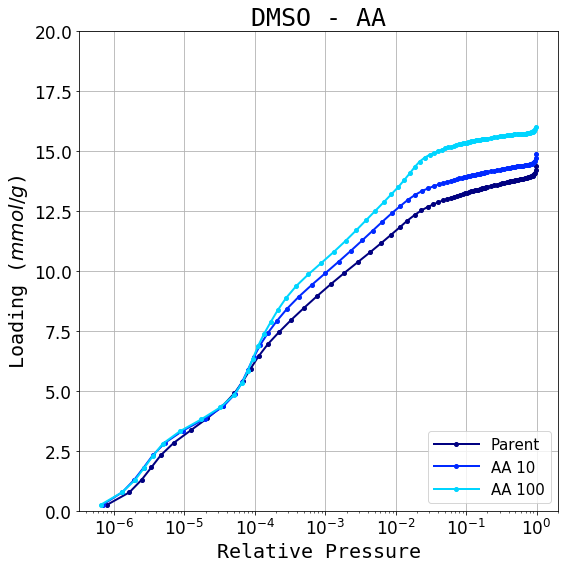
\includegraphics[width=\textwidth]{n2phys/dmso-aa}%
		\caption{}%
        \label{def:fgr:n2phys-dmso-aa}
    \end{subfigure}

    \caption{A selection of nitrogen sorption isotherms as measured on the
    leached samples: (a) formic acid in DMF, (b) trifluoroacetic
    acid in water, (c) benzoic acid in methanol and (d) acetic acid
    in DMSO. The curve for the parent material is in dark blue.}%
    \label{def:fgr:n2phys-dataset}
\end{figure}